%!TEX root = ../report.tex

\begin{document}
    \chapter{State of the Art}
    Methods for detecting a fault in signals can be classified into two types model-based approach and feature-based approach. In the model-based methods, a time-ordered stochastic process is used to describe the observations. This method is sensitive to noise and the fault model that describes the characteristic fault in signal must be defined. This information is generally not available in real-time data thus in such cases feature-based approaches are preferred. In this approach features are considered as random set variables and extracting features and selecting feature subsets are crucial steps. Which in turn reduces the number of attributes or data dimensions considered when making a decision. This work focuses on feature extraction of time series data and in the following sections detailed literature review is presented.
    \section{Feature extraction}
    The main goal of feature extraction is to reduce the dimensionality of data and retain important information of the original data. This method makes use of characteristics that are effective visual indicators of distinct populations and the physics that underpin them. The process of feature extraction reduces the redundant information and eliminates noise in-turn reducing the time for time-series classification. This approach is specifically built for discriminative models of classification where the relation between the time series features and probability distribution of classes is learned \cite{ismail2019deep}. There are various techniques available which are discussed in following sections. 
    \subsection{Domain specific methods}
    
    To analyze time series data both time domain and frequency domain methods are available. These features are handcrafted with help of the domain knowledge and then used as discriminators in classification models. Multiple features are required to model the data for classification, if only one feature is used it can lead to high uncertainty and misclassification of data. When the length of the signal is small, the time domain features suffice the analysis but as the length increases to reduce the dimensionality frequency domain features are suitable \cite{shumway2000time}. One of the early methods temporal features such as min, max and skewness were extracted for data as in \cite{nanopoulos2001feature}. In \cite{geurts2001pattern} the maximum and minimum peaks of the time series were extracted to observe the pattern in audio data. A fixed set of domain-specific features have been extracted for example time-domain features such as mean, variance etc. Statistical features are calculated from the raw data to create the compressed representation. Several papers suggest that these features can be used to recognize patterns in time series. Statistical features such as skewness, kurtosis and entropy can be used to classify audio signals in \cite{lambrou1998classification}.
    Feature extraction can be applied to whole data or by dividing it into windows and creating representation for each. There have been several studies that based the classification
    on the mean, standard deviation, skewness, and kurtosis of the time series \cite{nanopoulos2001feature}. A similar approach is defined in the Highly comparative feature-based method by \cite{fulcher2014highly}. -Different systems implement the highly comparative approach. Tsfresh \cite{christ2018time} is currently one of the most popular tools. The appropriate features are selected using the FRESH algorithm (Feature Extraction using Scalable Hypothesis tests). It performs the following tasks: '
    \begin{itemize}
    	\item Testing hypotheses to determine the level of dependency between each label and the target labels.
    	\item Features are selected based on p-values computed for each of them.
    	\end{itemize}
  Along with this approach to fuse data from multiple sensors and creating a feature vector a library named Tsfuse is present \cite{de2019automating}. Commonly used feature extraction in frequency domain is using Fast Fourier transform details of which have been described in chapter 3 and the application can be seen in paper \cite{gowid2015novel}. Another domain specific method which provides information on both domains is wavlet transform it eliminates drawbacks of conventional Fourier transform. It has been successfully implemented in \cite{joo2015time}  which provides promising results. 
  
  Main issue with the domain specific methods is generalization of the problem is difficult for example the features that work for ECG data might not be effective for sound signals.The process is time consuming and expensive to calculate. Another issue related to this kind of method is it requires labeled data sets which is sometimes not available in real time data.

    
     \section{Deep-learning}
    To overcome the short comings of the domain specific methods unsupervised learning algorithms can be applied for feature extraction \cite{bengio2007scaling}. Also the deep learning methods are comparatively better at modeling complex real time data. Deep networks are designed to separate the factors that affect input data variation at the lower layers and combine the representations at the higher layers. There are various deep-learning models that have been investigated for feature extraction of time series data most commonly used is Autoencoder as it can be seen in the paper \cite{kuznetsov2020electrocardiogram}. Many implementations such as \cite{mehtab2022analysis}, \cite{sagheer2019unsupervised} are available for modeling the data using LSTMs and Recurrent neural network(RNN) to model time-series data as these models are suitable for sequential data. The problem with RNNs is that they have difficulty in learning longterm defficencies due to the vanishing gradient problem \cite{hochreiter2001gradient} which can be solved by LSTMs. According to \cite{langkvist2014review} LSTMs are not that effective to model this type of data.
    \cite{ren2017novel} examined implementation of Deep Belief Network (DBN) on sensor data by Human activity recognition data \cite{vrigkas2015review}. The method presented here does not have a effective signal processing unit and the labels of data are ignored. To overcome the ignorance of patterns which was seen in DBN deep neural network architectures which is popularly used for image classification data can be used that is CNN \cite{yang2015deep}. This implementation states that CNN can serve as a competitive tool of feature learning and classification  in comparison to the sate of art feature engineering techniques.
    Overview of methods that can be used for feature engineering of signal data is shown in figure \ref{l01}.
     \begin{figure}[h]
     	\centering
     	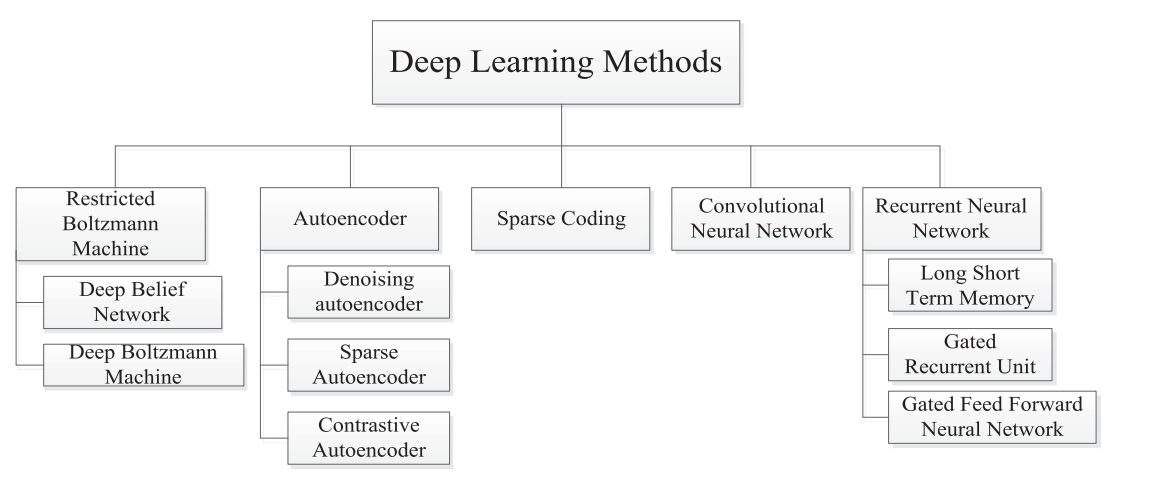
\includegraphics[width=1\linewidth]{images/dlm.png}
     	\caption{An overview of the different deep learning approaches for time series classification \cite{nweke2018deep}}
     	\label{l01}
     \end{figure}
     
     
     \section{Classification}
     The summary of classification algorithms is depicted in figure \ref{l0}. This thesis focuses on the Discriminative model of classification.
     
      \begin{figure}[h]
      	\centering
      	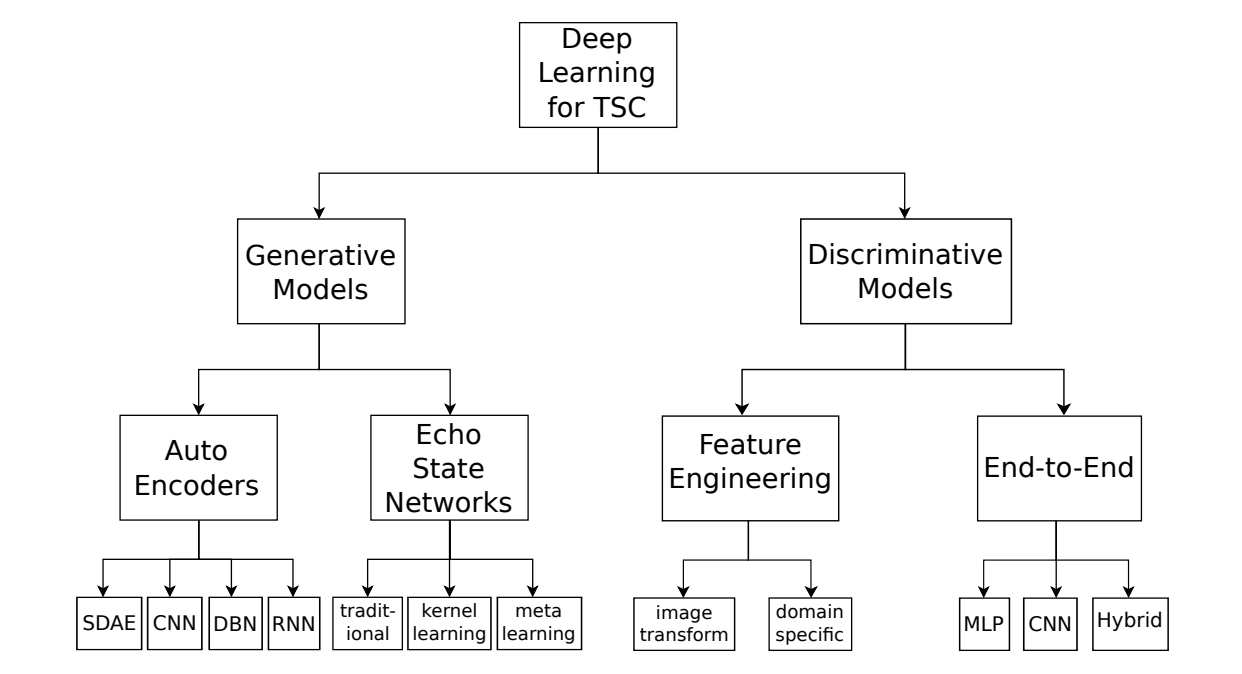
\includegraphics[width=1\linewidth]{images/tsc.png}
      	\caption{An overview of the different deep learning approaches for time series classification \cite{ismail2019deep}}
      	\label{l0}
      \end{figure}
     
     \subsection{Domain specific}
     Traditionally algorithms like 1-Nearest Neighbor algorithm is used in supervised classification environment \cite{bagnall2012transformation}. Most of the state of art machine learning techniques can be applied this problem when we conver the problem to feature space. 
    Convolution neural network have been gaining popularity in classification. Many variations of it are applied for this problem for example \cite{wang2017time}. 
     Inspired by natural language processing popular network such as AlexNet \cite{alom2018history} is applied for time series classification.
     
      \subsection{Image transforms}
      Instead of direct use of raw signal as input to the deep learning classifiers the signals can be encoded into two dimensional format. Many different approaches have been used to analyse and convert the signal in image format one of the poular is recurrence plots that help to analyse the next time step as can be seen in the implementation of \cite{thanaraj2020implementation}. Other types of image representations that have been reaserched are Gramian fields and  Markov transition fields \cite{wang2015imaging}.
      
      Another method of image transformation that uses both time and frequency domain information to represent the signal data is spectrogram which has been popularly used as input to classification for audio data. The implementation has also been effectively implemented for the human activity recognition data and ECG medical datasets.
      

   \subsection{Transfer learning}
  
  The major application for transfer learning model in time series data is done on medical dataset for example to detect abnormalities in ECG data \cite{o2021deep}. Major of the application transform  the signals into different image formats such as spectrograms due to many standard pretrained architectures exists for image data. For example Resnet \cite{ouyang2017audio} applied ot audio spectrograms and VGG \cite{russo2019classification} ECG dataset. 
  Most of studies present are for audio, medical and motion detection field. There are very few application that are done for acceleration signal data. Bench marked architectures are present for ECG data classification for example \cite{strodthoff2020deep}.  Similar to this \cite{yosinski2014transferable} provides a domain specific neural network designed for time series data.

  
  
    
    \chapter{Background Knowledge}
     \section{Feature extraction}
  
        \subsection{Domain-Specific Features}
     Standard machine learning classification algorithms cannot be directly applied to raw time series. Hence, features have to be extracted. As the concept of input and output features is missing in time series, variables should be chosen from it in such a manner that they aid to better classification of data. By evaluating the temporal relation between data points, time-domain processing better understands those relationships. If the information of interest repeats at regular or semi-regular intervals, a simple transformation can convert the time domain information to the frequency domain. This conversion isolates vibrational information for analysis within and between vibrational frequencies present in the time series. Following the domain, specific features can be extracted from the time-series data:
        
        \subsubsection{Temporal} 
        Temporal features define the ratios of relative intervals between events. The information about the frequency and sequence is not present in these features. These features are easy to extract and have simple physical interpretation, like: the maximum amplitude, minimum energy, centroid, mean absolute etc \cite{CakaNebi}.
         \subsubsection{Statistical} 
         These features are obtained by computing the statistic on the values of time-series. For example Kurtosis, Skewness, Maximum, Minimum, Mean, Median, etc.
         
          \subsubsection{Spectral} 
          These features can be obtained by converting the timeseries to frequency domain by using methods like Fourier transform. They help in analyzing patterns in the signal. For example fundamental frequency, frequency components, spectral centroid, spectral flux, spectral density, etc \cite{CakaNebi}.
        
    \subsection{Time domain transformations}
    Transforms in the time domain are similar to magnitude domain transformations, except they occur on the time axis. This means that the elements are displaced to different time step. There are various transformation described as follows
    
   
    
    \subsubsection{Slicing}
    Slicing of time-series is similar to cropping a image, that is either removing the end elements from the signal or selecting a particular pattern. This is represented in the figure \ref{l1}.
    This method can be used to select required information from the raw data or each slice from time series can be used in classification.
    
    \begin{figure}[h]
    	\centering
    	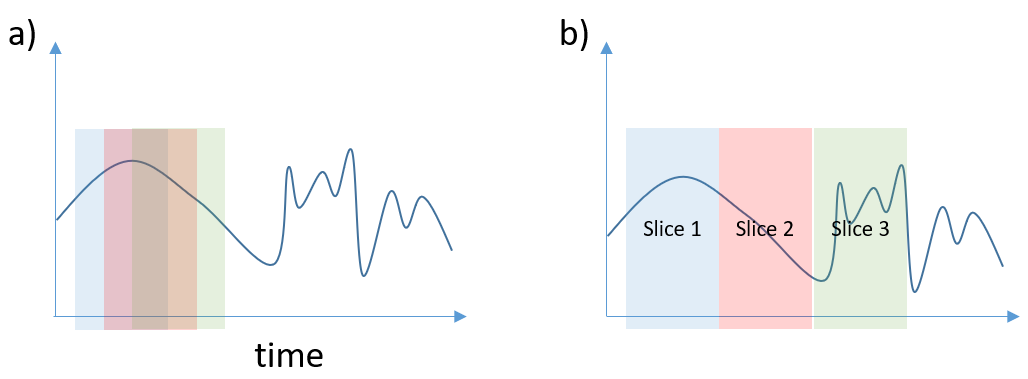
\includegraphics[width=0.75\linewidth]{images/MgfEa.png}
    	\caption{Window slicing \cite{le2016data}}
    	\label{l1}
    \end{figure}
    
    \subsubsection{Fourier transform}
    Fourier transform is a tool that converts the time-series  into alternate representation, characterized by the sine and cosine functions of varying frequencies. According to this theory any complex function can be represented as the combination of periodic functions which is known as Fourier series.
    \begin{equation}
    f(x) = \frac{a_0}{2}+\sum_{n=1}^{\infty}(a_ncos(\frac{2\pi n}{T}x)+b_nsin(\frac{2\pi n}{T}x)
    \label{e1}
    \end{equation}
    
      \begin{figure}[h]
      	\centering
      	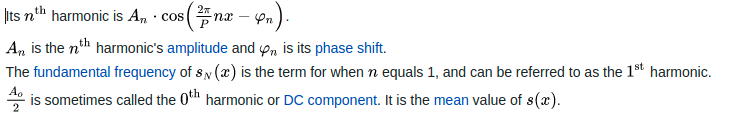
\includegraphics[width=0.75\linewidth]{images/fse.png}
    
      \end{figure}
    Any periodic time-series can be represented as sum of sinusoidal components which is given by the equation \ref{e1}. Time series is transformed into Fourier series by measuring every possible cycle and returning the amplitude, offset and rotational speed for every detected cycle. One of commonly used methods to achieve the transformations for real world signals is Fast Fourier transform (FFT). It is a optimized algorithm for obtaining Discrete fourier transform. A signal's frequency components are derived from sampled data over a period of time. Each component of a signal is a single sinusoidal oscillation with its own amplitude and phase.
    Figure \ref{l2} shows a example of transformation. 
    \begin{figure}[h]
        	\centering
        	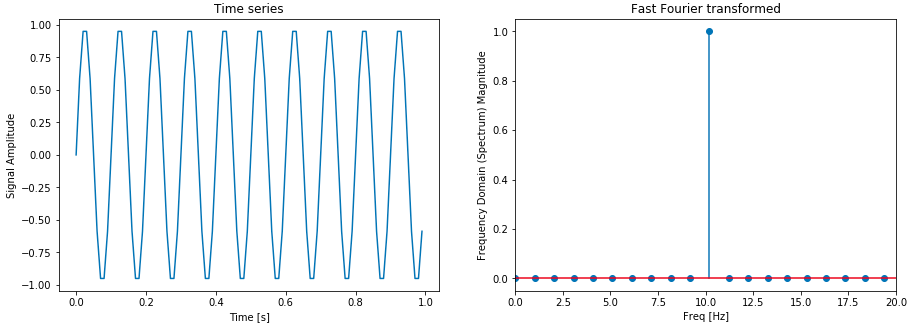
\includegraphics[width=0.75\linewidth]{images/fft.png}
        	\caption{Fast Fourier transform example \cite{imgfft}}
        	\label{l2}
    \end{figure}

    \subsubsection{Spectrogram Representation}
    Spectrogram is a visualization method where the temporal and spectral components of a signal can be viewed simultaneously. A spectrogram can be constructed using the short-time Fourier transform, that is a time window is determined, and then translated across the field. By calculating the Fourier transform of each windowed field, the spectrogram is created. As it provides a analysis of time-frequency simultaneously it can be used to identify the nonlinearities in signal. Thus it proves a important tool for analysis of real world data such as sound.  Figure \ref{l3} shows a example of spectrogram.
    
    \begin{figure}[h]
      	\centering
      	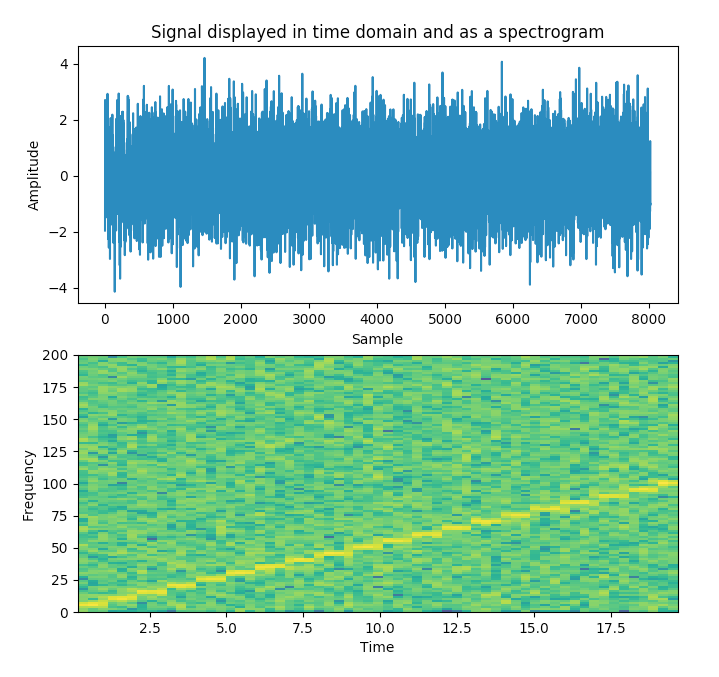
\includegraphics[width=0.5\linewidth]{images/spectrogram.png}
      	\caption{Spectrogram plot example \cite{spectrogram}}
      	\label{l3}
      \end{figure}
    Consider we have a signal x of length N. If we create consecutive segments of x having length of m where $m<<N $ and $X \in R^{m \times(N-m+1)}$ are the  consecutive columns of the matrix. That is, $ [x[0], x[1], . . . , x[m - 1]]^T$ is the first column $[x[1], x[2], . . . , x[m]]^T$ is second and so on. The rows and colums of this matrix are indexed by time. As we can observe that matrix X is repetitive representation of x.  
     So the spectrogram of signal is calculated by applying DFT to the columns of $X$  and obtaining a matrix $\hat{X}$. Therefore,
     \begin{gather}
     \hat{X} = \bar{F}X\\
     X = \frac{1}{m} F \hat{X}
     \end{gather}
    
 In the matrix  $\hat{X}$ columns are indexed by time and rows by frequency. So each value is representation of a point in frequency and time.  $\hat{X}$ is invertible due to the transformations performed above. The information in this matrix is also highly redundant. The matrix is spectrogram and can be visualized with help of a plot.

    

    \subsection{Deep-learning based methods }
    \subsubsection{Auto-encoder}
    Autoencoders are type neural networks which learn data encodings in unsupervised way. The network consists of two parts encoder and decoder. This encoder-decoder system learns efficiently through optimization process, that is when the data is fed to the network its output is compared to initial data and the error is backpropagated through the architecture to update the weights at each iteration. Three components of the autoencoder as seen in figure \ref{l4} are described as follows:
    \begin{enumerate}
    	\item \textbf{Encoder}: In this module the input data is converted to encoded representation by reducing the dimensionality of data. In terms of neural networks the encoding is accomplished by reducing nodes in subsequent layers.
    	The process reduces the information and only the most relevant or average information is forwarded.
    	\item \textbf{Latent space}: This space contains the reduced or compressed knowledge of the data. The representation obtained can be used as feature input to classification algorithms.
   	
    	\item \textbf{ Decoder}: This module reconstructs the encoded information of the data to it original, that is it decompresses the data.  
    \end{enumerate}
    
     \begin{figure}[h]
     	\centering
     	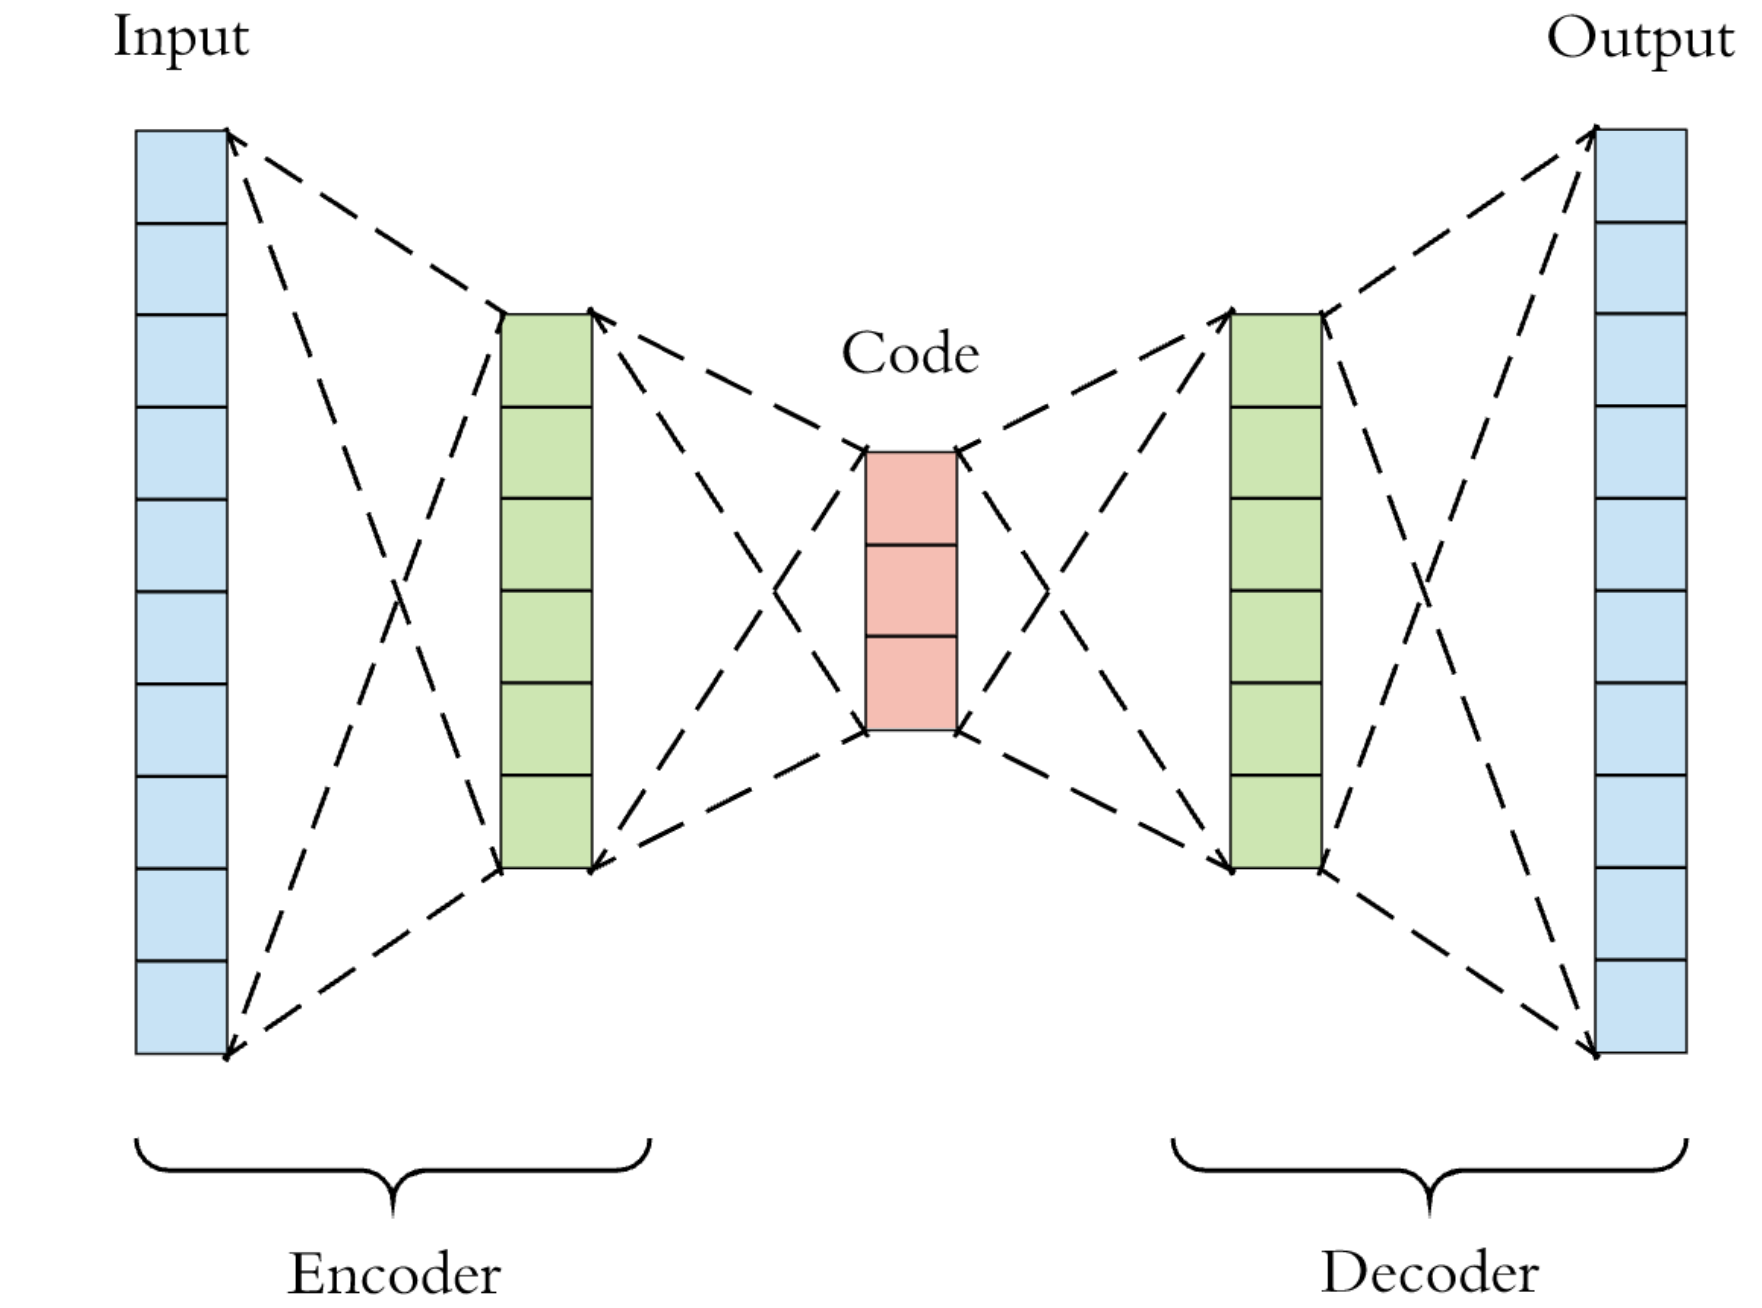
\includegraphics[width=0.6\linewidth]{images/auto.png}
     	\caption{Autoencoder \cite{auto}}
     	\label{l4}	
     \end{figure}
As discussed above the objective of autoencoder is to have input to be equivalent to output. The encoder function $\phi$ maps the data to latent space $F$ and decoder function $\varphi$ maps it back to original data $\chi$ as shown in following equations:
\begin{gather}
\phi: \chi \to F \\
\varphi : F\to \chi\\
\phi ,\varphi =arg min\left \|\chi -(\phi \cdot \varphi )\chi  \right \|^2
\end{gather}

The encoder network is modeled by passing the standard neural network function into activation function given in by equation \ref{e5}.$z$ here represents latent dimension
\begin{equation}
z=\sigma (Wx+b)
\label{e5}
\end{equation}

The decoder function can be represented similarly with help of different set of weights and biases and activation function.
\begin{equation}
x'= \sigma'(W'z+b')
\label{e6}
\end{equation}

The loss function can be written as:
\begin{equation} 
L(\mathbf{x}, \hat{\mathbf{x}}) = \mathbf{MSE}(\mathbf{x}, \hat{\mathbf{x}}) = \|  \mathbf{x} - \hat{\mathbf{x}} \| ^2 =  \| \mathbf{x} - \hat{\sigma} \{ \hat{\mathbf{W}} \left[\sigma ( \mathbf{W}\mathbf{x} + \mathbf{B} )\right]  + \hat{\mathbf{B}} \} \| ^2 \end{equation}
There are various implementation available for feature extraction using this method to encode the features of data instead using hand crafted method \cite{gerazov2018variational}. The deep autoencoders are designed in a fashion to reduce the dimensionality of raw sensor data \cite{ravi2019current} and transform them into feature vector with consized information on data. Variation of implementations can be found in the literature with a aim to find robust representation of data.
    \subsubsection{Long Short Term Memory networks(LSTM)}
    Long short-term memory (LSTM) is an artificial recurrent neural network (RNN) architecture used in the field of deep learning. Unlike standard feedforward neural networks (like CNN), LSTM has feedback connections. Because of the feedback connections, LSTM can not only process single data points (like image) but also a sequence of data points like a sentence or a time series. 
    
    A common LSTM unit is composed of a cell, an input gate, an output gate and a forget gate. The cell remembers values over arbitrary time intervals and the three gates regulate the flow of information into and out of the cell.
    In the image below, the $C_t $ is the cell state and it runs down the information through the entire chain. On this, the information is removed or added by Forget gate or Input gate. 
    \begin{enumerate}
    	\item The Forget gate: The first step in LSTM is to decide what information to remove from the cell state. This decision is made by a sigmoid layer called the forget gate layer. It looks at $h{t-1}$  and xt and outputs a number between $0$ and $1$  for each number in the cell state $C_{t-1} $ . A $1$ represents completely keep this while a $0$  represents completely get rid of this. The output of the forget gate is calculated using the following equation: 
    	 \begin{equation}
    	 f_t=\sigma(W_f.[h_{t-1},x_{t-1}]+b_f)
    	 \end{equation}
    	 \item Input gate: The next step is to decide what new information we are going to store in the cell state. For this step, first the sigmoid layer decides which values to update. Then a $tanh$ layer creates a vector of new values that are to be added in the cell state. Then these two are combined to create an update to the state. Mathematically it represented by: 
    	 \begin{gather}
    	 i_t=\sigma (W_i.[h_{t-1},x_{t-1}]+b_i)	\\		
    	 C_t=tanh(Wc.[h_{t-1},x_{t-1}]+b_c)
    	 \end{gather}
    	 The updated cell state is calculated by: $C_t=f_t*C_{t-1}+i_t*\bar{C}_t$
    	 \item Output gate: In the next step, the output is calculated. This will be a filtered version of the cell state. First, a sigmoid layer is used which decides what parts of the cell state are going to output. Then, the cell state is put through $tanh$ (to push the values to be between $-1$ and $1$ ) and multiply it by the output of the sigmoid gate, so that only the decided parts are output. Mathematically it is represented as: 
    	  \begin{gather}
    	o_t=\sigma (W_o[h_{t-1},x_{t-1}]+b_o)\\				
    	h_t=o_t*tanh(C_t)
    	  \end{gather}
    	 
    \end{enumerate}
 
 In the above equations, the lowercase variables represent vectors. Matrices Wq contains the weights where the subscript q can either be the input gate i, output gate o, the forget gate f or the memory cell c, depending on the activation being calculated. A vector notation was used which means ctRh is not just one unit of one LSTM cell, but contains $h$ LSTM cell's units.
 
   \begin{figure}[h]
   	\centering
   	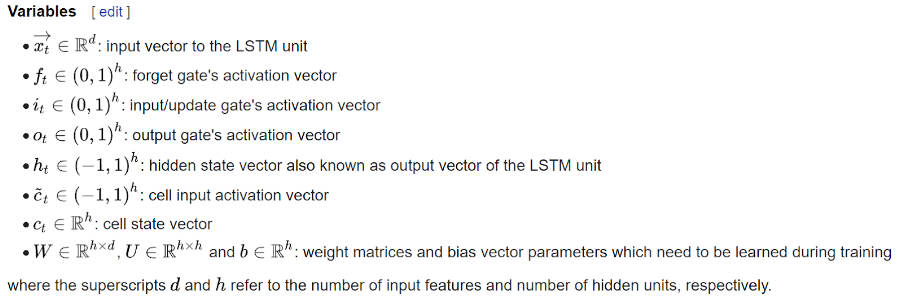
\includegraphics[width=1\linewidth]{images/vv.png}

   
   \end{figure}
   
   \begin{figure}[h]
   	\centering
   	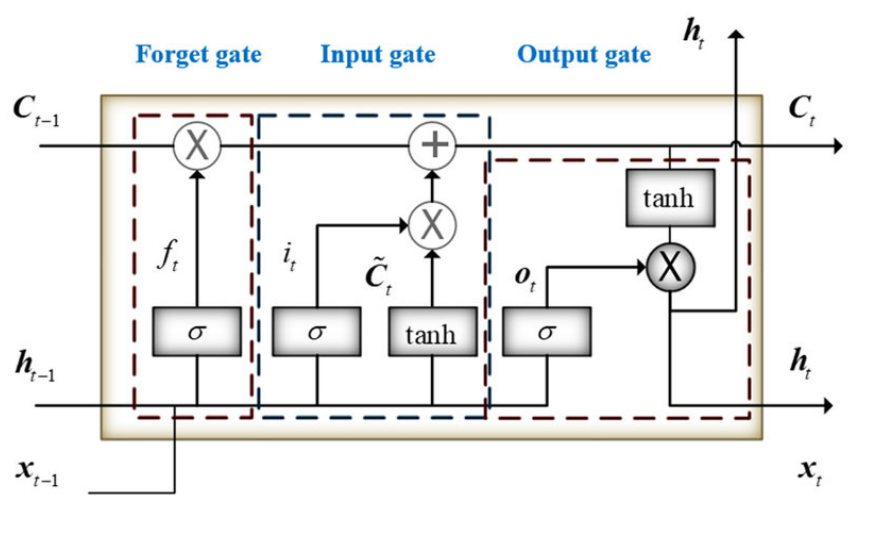
\includegraphics[width=0.6\linewidth]{images/lstm.png}
   	\caption{The repeating module in an LSTM}
   	\label{l6}	
   \end{figure}
   
 
    \subsubsection{CNN}
    A Convolutional Neural Network (ConvNet/CNN) is a Deep Learning algorithm which is most commonly applied to analyse visual imagery. The architecture of a ConvNet is analogous to that of the connectivity pattern of Neurons in the Human Brain and was inspired by the organisation of the Visual Cortex. In humans, Individual neurons respond to stimuli only in a restricted region of the visual field known as the Receptive Field. The receptive fields of different neurons partially overlap such that they cover the entire visual field.
    
    As compared to multilayer perceptron (fully connected networks in which each neuron in one layer is connected to all neurons in the next layer), CNN takes advantage of the hierarchical pattern in data. They assemble the patterns of increasing complexity using smaller and simpler patterns embossed in their filters. Therefore, on a scale of connectivity and complexity, CNNs are on the lower extreme. CNNs use relatively little pre-processing compared to other image classification algorithms. This means that the network learns to optimise the filters (or kernels) through automated learning, whereas in traditional algorithms these filters are hand-engineered.
    
    A CNN consists of the input layer, the hidden layer and the output layer. The hidden layer of a CNN consists of convolution layers, pooling layers and fully connected layers. 
    Input layer: the input layer of a CNN is a tensor of the image with a shape: (number of inputs) x (input height) x (input width) x (input channels).
    Hidden layer: 
    \begin{enumerate}
    	\item Convolution layer: The element involved in carrying out the convolution operation in the Convolutional Layer is called the Kernel/Filter. The filter slides over the input matrix with a certain Stride Value and at each step a dot product is performed. Filter moves to the right till it parses the complete width. Moving on, it hops down to the beginning (left) of the image with the same Stride Value and repeats the process until the entire image is traversed. This process generates a feature map which is the input to the next layer. In a CNN, multiple convolution layers are present and at each convolution layer, the feature map complexity increases. 
    	\item Pooling layer: Pooling layers reduce the dimensions of data by combining the outputs of neuron clusters at one layer into a single neuron in the next layer. Furthermore, it is useful for extracting dominant features which are rotational and positional invariant, thus maintaining the process of effectively training the model. 
    \end{enumerate}
       
    The Convolutional Layer and the Pooling Layer together form the i-th layer of a Convolutional Neural Network. Depending on the complexities in the images, the number of such layers may be increased for capturing low-level details even further, but at the cost of more computational power. 
    After going through these layers, the input image is converted into a suitable form for Multi-Level Perceptron (Fully connected layer). The image is flattened into a column vector and  is fed to a feed-forward neural network and backpropagation applied to every iteration of training. Over a series of epochs, the model is able to distinguish between dominating and certain low-level features in images and classify them using the Softmax Classification technique.
      \begin{figure}[h]
      	\centering
      	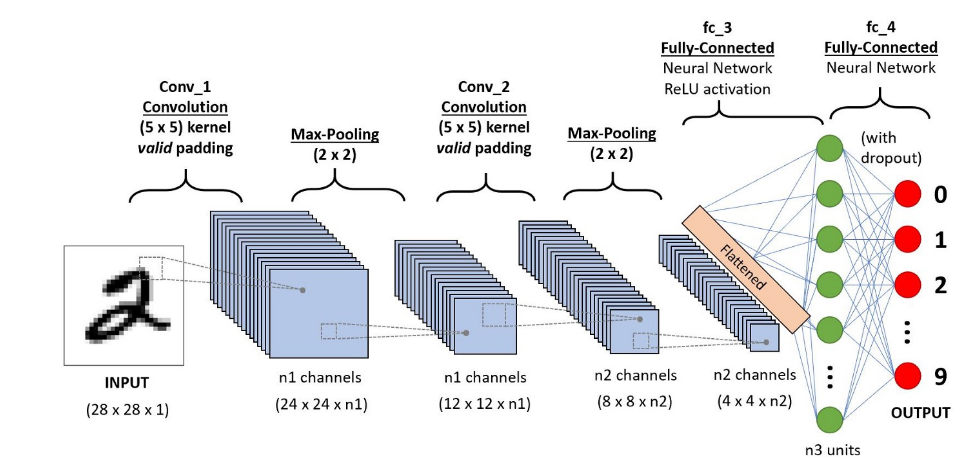
\includegraphics[width=1\linewidth]{images/cnn.png}
      	\caption{CNN architecture for image classification \cite{imgcnn}}
      	\label{l00}	
      \end{figure}
    
    \subsection{Transfer-learning}
    A transfer learning method is a machine learning approach that reuses a model developed for one task as a starting point for a second model. Usage of pre-trained models is widely used as they can be used as a start point for solving computer vision or natural language processing tasks. The reason is that developing neural network models for these tasks requires significant amount of computation and time resources. There are two ways to apply transfer learning models described as follows:
    
    \subsubsection{Develop Model Approach}
    \begin{enumerate}
    	\item First step in this approach is to select predictive model such that is trained with large amount of data. Also there should be some relation between the data we want to implement this model for and the concept for which the model is trained.
    	\item After completing the first task, you need to develop an effective model. There must be some feature learning done in the model compared with naive models.
    	\item Modeling the second task of interest can then be based on the model fit on the source task. The model may be used in its entirety or in parts, depending on the modeling method used.
    	\item  In some cases, the model may need to be customized or refined according to the input-output pairs available for the particular problem at hand.
    \end{enumerate}
    \subsubsection{Pre-trained Model Approach}
     \begin{enumerate}
     	\item From the available models, a pre-trained model can be selected. There are many sources available from research institutions from where a model can be selected according to the problem requirements.
     	\item After finding a suitable model it can be used as a starting point for second task. Depending on the task a part of model or the entire model can be used.
     
     	\item  Lastly, the model may need to be customized or refined according to the input-output pairs available for the particular problem at hand.
     \end{enumerate}
    
    For this project the transfer-learning is done by using spectrogram as input because the comfort door data is a complex industrial data.
    
    \subsection{Transfer-learning models for images}
   
   
    \subsubsection{VGG}
    As it can be visualized in the figure \ref{l05} this network uses a simple design by stacking 3×3 convolutional layers in depths of increasing magnitude. This network uses max pooling to reduce volume size. Two fully-connected layers, each with 4,096 nodes are then followed by a softmax classifier \cite{simonyan2014very}. 
    According to findings of \cite{simonyan2014very} in 2019 the network was too deep hence hard to train. Thus to make the process of training easier the concept of pre-training is used. In this process step by step training was output of smaller networks was fed to larger as initial step and so on so forth. 
    Even though the pre traing is a logical step it is a tedious task and requires large computation time.
    
     \begin{figure}[h]
     	\centering
     	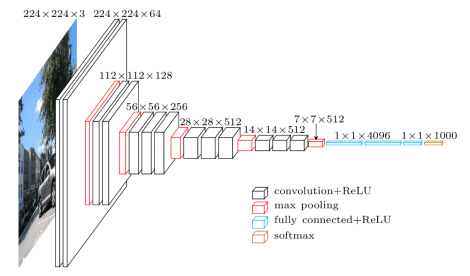
\includegraphics[width=0.8\linewidth]{images/imagenet_vgg16.png}
     	\caption{VGG network architecture \cite{simonyan2014very}}
     	\label{l05}	
     \end{figure}
    
    Disadvantage of using VGG are as follows:
    \begin{enumerate}
    	\item It trains very slowly
    	\item In terms of bandwidth the weights of network are very high.
    \end{enumerate}
    
 \subsubsection{Resnet}
 With the increase in depth of layers the training becomes a tedious task as seen in section above. Also with the depth there the networks face vanishing gradient problem a problem. As a result the performance gets saturated along the depth. Therefore to solve this problem Resnet provides a identity shortcut connection that is, it skips one or more layers as can be seen in figure \ref{ll}. 
      \begin{figure}[h]
      	\centering
      	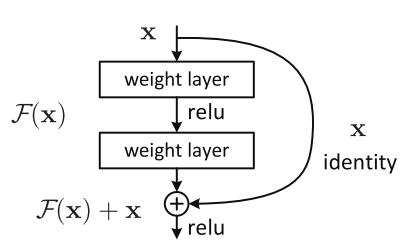
\includegraphics[width=0.5\linewidth]{images/resd.png}
      	\caption{Residual learning: a building block \cite{he2016deep}}
      	\label{ll}	
      \end{figure}
     
            
The advantage of using the skip layer is if a layer affects the performance of the network it is skipped. The basic idea behind the skip layer is that it is easier to learn the value of $F(x)$  to be zero so it acts like identity function rather than learning the identity function. So this block is also known as the identity block.
Another element of the residual network is convolution block.  These blocks help in reshaping the output from the first layer to the third layer. Both of these components of Resnet help it in gaining high accuracy and optimization level. 

       \begin{figure}[h]
       	\centering
       	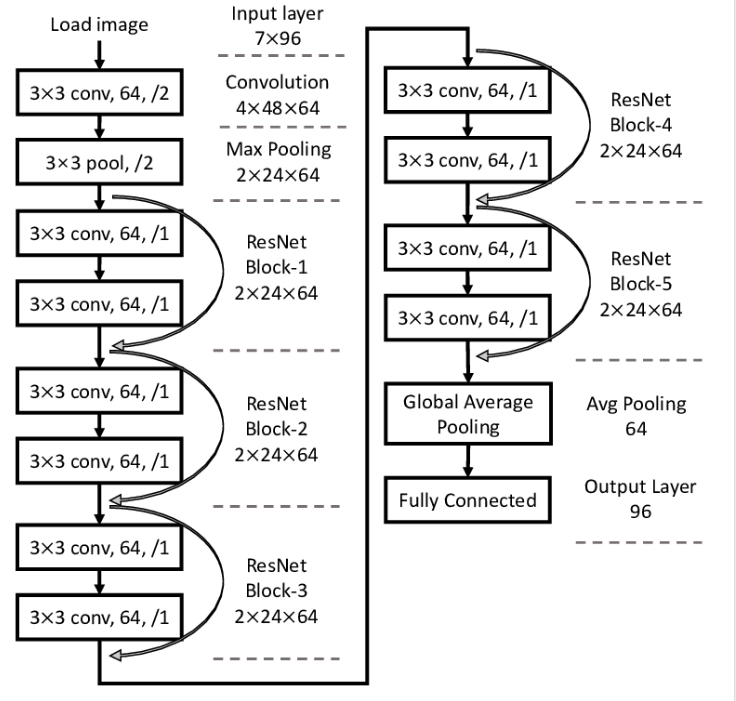
\includegraphics[width=0.5\linewidth]{images/rs.png}
       	\caption{Resnet architecture \cite{inproceedings}}
       	\label{ll1}	
       \end{figure}

\end{document}
